\documentclass[11pt,a4paper]{article}
\usepackage[utf8]{inputenc}
\usepackage[T1]{fontenc}
\usepackage[polish]{babel}
\usepackage{lmodern}
\usepackage{graphicx}
\usepackage{epstopdf}
\usepackage{anysize}
\usepackage{makeidx}
\usepackage{hyperref}



\makeatletter
\renewcommand{\maketitle}{
\begin{titlepage}
\begin{center}

\LARGE{AKADEMIA GÓRNICZO-HUTNICZA}

\vspace*{1cm}

\includegraphics[scale=1.8]{agh.eps}
\vspace*{1cm}

\LARGE{im. Stanisława Staszica w Krakowie}

\rule{\textwidth}{0.4mm}
\LARGE \textsc{\@title}
\rule{\textwidth}{0.4mm}

\vspace*{5mm}

% Author and supervisor
\begin{minipage}{0.4\textwidth}
\begin{flushleft} \large
\emph{Autorzy:}\\
Bartłomiej \textsc{Bułat}\\
Tomasz \textsc{Czarnik}\\
Krzysztof \textsc{Śmiłek}\\
\end{flushleft}
\end{minipage}
\begin{minipage}{0.4\textwidth}
\begin{flushright} \large
\emph{Opiekun projektu:} \\
dr inż.~Mirosław \textsc{Jabłoński}
\end{flushright}
\end{minipage}
\vfill
\vspace*{\stretch{8}}
\rule{\textwidth}{0.4mm}

\large{Wydział Elektroniki, Automatyki, Informatyki i Elektrotechniki}\\
\large{Katedra Automatyki}\\
\large{Laboratorium Biocybernetyki}\\
\vspace*{\stretch{7}}
\@date

\end{center}

\end{titlepage}
}
\makeatother

\title{Lokalizacja twarzy na obrazie za pomocą konwolucyjnych sieci neuronowych}
\date{\today}

\makeindex

\begin{document}

\maketitle

\newpage

\tableofcontents

\newpage

%=================================================
\section{Streszczenie}

Celem naszego projektu jest zbudowanie prototypu systemu pozwalającego na detekcję twarzy na obrazie 
w oparciu o sieć neuronową typu CNN (Convolutional Neural Network).
%=================================================
\section{Wstęp}

\subsection{Co to jest sieć neuronowa?}
Siec neuronowa jest modelem matematycznym składającym się z sieci węzłów obliczeniowych zwanych neuronami
 i ich połączeń. Jest to pewna technika obliczeniowo-statystyczna, należąca do dziedziny sztucznej inteligencji. 
Jej zadaniem jest symulacja działania ludzkiego mózgu. 

\subsection{Budowa sieci neuronowej}
Nasz mózg jest zbudowany z ogromnej ilości neuronów które komunikują się ze sobą za pomocą impulsów elektrycznych.
 Z informatycznego punktu widzenia neuron stanowi układ przetwarzający pewne dane, posiadający wiele wejść
 oraz jedno wyjście. Oto porównanie neuronu naturalnego ze sztucznym:

\vspace*{1cm}
\begin{center}
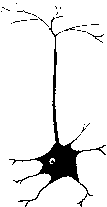
\includegraphics[scale=0.7]{neuron}
\hspace*{1cm}
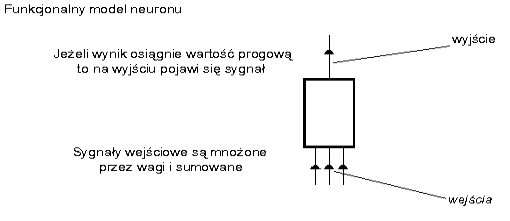
\includegraphics[scale=0.7]{neuron2}
\end{center}
\vspace*{1cm}

Działanie sztucznego neuronu można opisać w przybliżeniu następująco:\\
Sygnały $x_{i}$ podane na wejścia są mnożone prze odpowiednie wagi $w_{i}$ oraz sumowane. Wagi mogą 
przyjmować dowolne wartości rzeczywiste. Zakłada się, że $x_0 = 1$, więc $w_0$ jest stałym
pobudzeniem neuronu. Równanie neuronu wygląda zatem następująco:

\begin{center}
$Y = x_0w_0 + x_{1}w_{1} + x_{2}w_{2} + x_{3}w_{3} + … + x_{n}w_{n} + b$\\
\end{center}

Suma ta staje się następnie argumentem funkcji aktywacji, która zwykle zwraca wartości z zakresu 
$(-1,1)$. Wynik tej funkcji pojawia się zarazem na wyjściu z neuronu.\\
\\
Jak możemy zauważyć pojemność pojedynczego neuronu nie jest duża, a więc nie może on zapamiętać 
zbyt dużej ilości wzorców. Aby tego dokonać należy połączyć wiele pojedynczych neuronów w sieć. 
Dokonuje się tego tworząc kolejne warstwy. Czym więcej warstw tym sieć bardziej złożona. Ilość 
neuronów w poszczególnych warstwach może się różnić i zależy od konkretnego zastosowania sieci. 
Należy do tego dodać, że neurony w jednej warstwie nie są połączone ze sobą, natomiast neurony z
dwóch sąsiednich warstw są połączone "każdy z każdym". Sygnał przechodzi do warstwy wejściowej 
poprzez ukrytą aż do wyjściowej, skąd jest odbierany i interpretowany.

%=================================================
\section{Proponowane rozwiązanie}
\subsection{Lokalizacja twarzy za pomocą CNN}

\vspace*{1cm}
\begin{center}
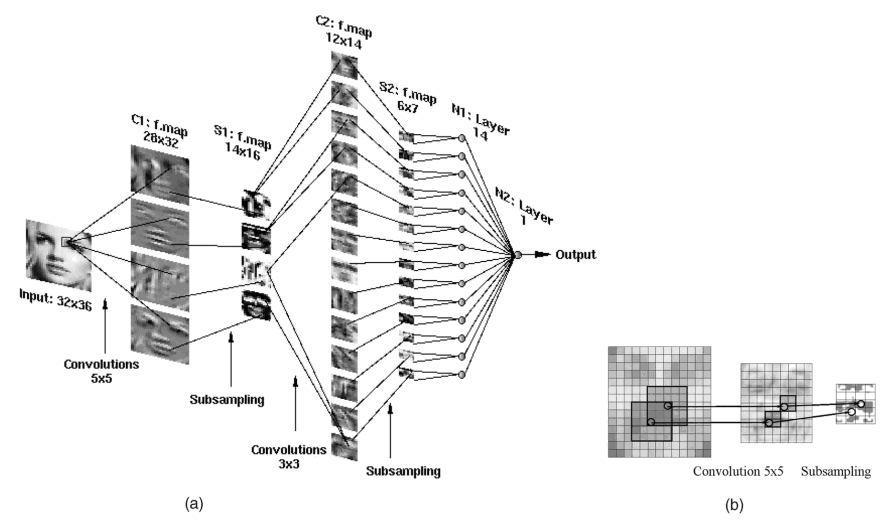
\includegraphics[scale=0.7]{schemat}
\end{center}
\vspace*{1cm}

Sieć ta składa się z sześciu warstw. Pierwsze 4 to naprzemian warstwy konwolucyjne (\textbf{C}) i 
warstwy subsamplingu (\textbf{S}). Ostatnie dwie to warstwy zwykych neuronów (\textbf{N}). Sieć jest 
zaprojektowana tak, żeby mogła przetwarzać obrazy większe niż 32x36 pikseli.

Warstwy od \textbf {C1} do \textbf{S2} składają się z skupisk neuronów które przeprowadzają operacje
konwolucji lub subsamplingu na wyjściach z wyższych warstw. Skupiska te są nazywane inaczej mapami
cech, ponieważ każde z nich wydobywa z obrazu wejściowego inną cechę. Warstwa  \textbf{N1} zawiera 
szereg niezależnych od siebie neuronów podłączonych wyjściami do \textbf{N2}, która jest zarazem
zakończeniem całej sieci neuronowej. Każdy element w danej warstwie otrzymuje na wejście informacje 
od małego zbioru elementów z warstwy poprzedniej. Koncepcję te pokazano na rysunku  \textbf{(b)}.

Postaramy się teraz opisać dokładniej poszczególne elementy tworzące  przedstawioną powyżej
architekturę sieci neuronowej. Różne parametry opisujące całą sieć tj. ilość warstw, ilość elementów
w warstwie, rodzaj połączeń między nimi a także wielkość poszczególnych elementów została wybrana 
doświadczalnie przez C. Garcia i  M. Delakis. Przetestowali oni szeroki zakres wielu architektur 
sieci i przedstawiona powyżej okazała się najbardziej skuteczna zarówno pod względem wykrywalności 
twarzy jak i odporności na zakłócenia obrazu.
 
Warstwa  \textbf {C1} jest złożona z czterech map cech. Każda mapa jest wynikiem konwolucji obrazu 
wejściowego z maską 5x5 powiększoną o stałe pobudzenie neuronu (bias), dlatego wyjściowy obraz jest 
mniejszy od wejściowego o 4 piksele (piksele brzegowe są odrzucane). Wartości maski oraz stałe 
pobudzenie mogą ulec zmianie w trakcie treningu. Podsumowując, w warstwie tej znajduje się 
104~($4  \cdot 26$) trenowanych zmiennych.

Warstwa  \textbf{S1} złożona jest z czterech map cech, każda połączona z jedną mapą cech warstwy 
wyższej. Każda z map powstała poprzez przeskalowanie wejścia, zmniejszając je dwukrotnie (Jako 
wartość nowego piksela przyjmowana jest średnia pikseli sąsiednich). Zmniejszony obraz jest mnożony 
przez wagę i powiększany o bias. Obie zmienne mogą ulec zmiane podczas treningu. Wynikowy obraz jest
argumentem do funkcji aktywacji (tangensa hiperbolicznego). Funkcja ta wprowadza nielinowość do 
modelu sieci neuronowej. Podsumowując, w warstwie \textbf{S1} znajduje się 8~($4 \cdot 2$) 
trenowalnych parametrów.

Jak można zauważyć na rysunku  \textbf{(a)}, kolejne warstwy składają się z coraz większej ilości 
map cech, ale za to ich rozdzielczość się zmniejsza. Taki rodzaj systemu sieci został zaproponowany 
przez Hubela i Weisela i dobrze wyodrębnia on z obrazu cechy potrzebne do poźniejszego przetwarzania
przez neurony.

Warstwa  \textbf{C2} to konwolucyjna warstwa z 14 mapami cech. Pierwsze 8 powstało w wyniku
konwolucji z maską 3x3 map z poprzedniej warstwy. Pozostałe 6 to złożenia dwóch z czterech map z 
warstwy \textbf{S1} (co wynika z wzoru na ilość kombinacji: $4 \choose 2$ $ = 6$).\\
Oto schemat przykładowego złożenia map o numerach 1 i 4:

\begin{center}
$Y = maska^{(1)}_{3x3}*mapa_{1}+maska^{(2)}_{3x3}*mapa_{2}+bias$
\end{center}

Podsumowując, warstwa ta składa się z 14 map cech oraz z 196~($8 \cdot (3 \cdot 3+1) + 6 \cdot (2 
\cdot 3 \cdot 3 +1)$) trenowalnych zmiennych.

Warstwa  \textbf{S2} to warstwa subsamplingu analogiczna do warstwy  \textbf{S1}. Składa się ona z
14 map cech oraz 28 ($14 \cdot 2$) trenowalnych zmiennych.

Ostatnie 2 warstwy składają się juz ze zwykłych neuronów. Ich zadaniem nie jest ekstrakcja cech jak 
miało to miejsce w poprzednich warstwach, ale ich klasyfikacja. W  \textbf{N1} każdy z pojedynczych 
neuronów jest w pełni połączony z obszarem 6x7 pikseli (co w przypadku obrazów uczących pokrywa się 
z wyjściem poprzedniej warstwy) tylko jednej odpowiadającej mu mapy cech z \textbf{S2}. Natomiast w 
warstwie  \textbf{N2} istnieje tylko jeden neuron, który łączy się z wyjściami ze wszystkich 
neuronów z \textbf{N1}. W przypadku gdy na wejście podany jest obraz jest większy od obrazu 
uczącego, neurony przetwarzają każdy fragment osobno produkując na wyjściu macierz odpowiedzi.

Wszystkie neurony z warstw  \textbf{N1} i  \textbf{N2} wykonują klasyczny iloczyn skalarny pomiędzy 
wektorem wejściowym, a wektorem wag, do czego później dodawany jest bias. Wynik sumy jest argumentem
funkcji aktywacji (tangensa hiperbolicznego), dlatego na wyjściu otrzymujemy liczbę z zakresu 
$(-1,1)$. Wyjście z ostatniej warstwy  \textbf{N2} jest używana do klasyfikacji obrazu jako twarz 
(wynik większy od zera) lub nie-twarz (w przeciwnym przypadku). Warstwy  \textbf{N1} i  \textbf{N2} 
mają odpowiednio 602~($14 \cdot (4 \cdot 7 + 1)$) i 15 trenowalnych zmiennych.

\subsection{Trenowanie sieci}

Stworzyliśmy zestaw szkoleniowy wybierając ponad 2500 obrazków zawierających twarze i nie-twarze. 
Zdjęcia pozyskaliśmy z internetowych baz danych które udostępniały twarze w różnych perspektywach. 
Naszym zadaniem było ich wyselekcjonowanie i odpowiednie przycięcie, tak by do sieci neuronowej 
wprowadzić jasno i czytelnie które zdjęcia powinien zakwalifikować jako twarz, a które nie. Zdjęcia 
staraliśmy się także dobierać w ten sposób aby skutecznie wyłapać różne cechy na obrazach, tak aby 
nasz system stał się jak najbardziej niezawodny i aby wykrywał twarze z jak największą 
skutecznością.

Sam proces przycinania obrazków polegał na tym, aby obrazek przeskalować, bądź przyciąć do wielkości
32x36px. Przy czym głównym celem było to, aby usta i oczy wybranych osób znajdowały się na każdym 
obrazie mniej więcej w tym samym miejscu. Odległość pomiędzy ustami, a oczami jest znacząca, 
ponieważ pozwala ona na zachowanie odpowiednich proporcji twarzy. Proporcje te to: odległość między 
oczami około 16px, a między oczami i ustami 18px.

Zbieranie zbioru nie-twarzy okazało się o wiele trudniejsze niż sądziliśmy. Praktycznie każdy obraz 
nie zawierający twarzy mógłby posłużyć jako obraz testowy. Jednak w tym wypadku proces testowania 
jest mniej dokładny. Większą dokładność uzyskuje się podczas testowania obrazków które nie są 
twarzami, ale je znacząco przypominają. Jednak taki zbiór obrazów jest z oczywistych względów bardzo
trudny do pozyskania, przez co posłużyliśmy się do testów obrazami losowo wyciętymi z większych 
zdjęć przedstawiających krajobrazy. 


Sam proces trenowania przedstawia się natomiast w następujących krokach:
 \begin{enumerate}
\item Stworzenie zbioru 400 obrazów przedstawiających twarz i 400 nie zawierających jej.
\item Ustawienie zmiennych: BootsIter = 0
\item Wybranie spośród zbioru utworzonego w (1) twarzy po 300 obrazów z twarzą i 300 bez.
\item Trenowanie sieci przez około 10 trenowalnych epok. W każdej epoce używana jest taka sama 
liczba pozytywnych i negatywnych przykładów. Trenowanie odbywa się natomiast metodą wstecznej 
propagacji błędów ze współczynnikiem uczenia (od 0.005)
\item Inkrementacja zmiennej BootsIter = BootsIter+1;
\item Jeśli BootsIter < 6 to idź do (3)
\item Trenowanie sieci przez kolejne 10 epok, ale już dla całego zbioru obrazów.
 \end{enumerate}

Przedstawiony wyżej algorytm został dokładniej opisany w artykule [1]. 
Oryginalnie algorytm zawierał również zmienną określającą wartość od której zbierane są tzw. 
fałszywe alarmy (negatwyne przykłady, dla których dostaliśmy pozytywną odpowiedź). Sposób zbierania 
tych przykładów i ich wykorzystania do nauki był dość zawiły, a także nie wpływał na jakość uczenia
się sieci, dlatego opuściliśmy go w naszej implementacji.

\subsection{Testowanie}

Proces testowania rozpoczęliśmy wykonując wcześniej wspomniany algorytm krok po kroku. Jednakże 
podczas nauki za pomocą metody wstecznej propagacji błędów zauważyliśmy, że nauka ta nie przynosi 
żadnych rezultatów.

Po konsultacji z prowadzącym doszliśmy do wniosku, że wina najprawdopobobniej leży w tym, że twarz 
jest dosyć skomplikowanym obiektem, o mnóstwie cech. Postanowiliśmy zatem, że zamiast wykrywać 
twarze będziemy wykrywać na obrazach cyfry, które są prostsze do opisania, ponieważ posiadają 
mniejszą liczbę własności. Ponownie zatem stworzyliśmy bazę obrazów z cyframi i wykonaliśmy 
wspomniany algorytm dla nowych danych. Dla tej samej budowy sieci program zaczął rozróżniać cyfry.

Wykres uczenia się systemu dla przeprowadzonych testów prezentuje się następująco:
\begin{center}
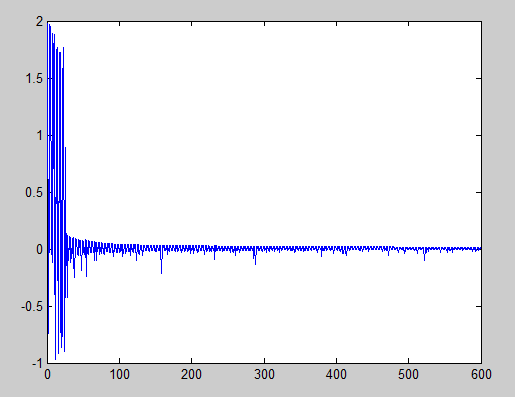
\includegraphics[scale=0.5]{wykres}
\end{center}

Jak możemy zauważyć, z każdą przeprowadzoną iteracją wartość błędu obliczeń się zmniejsza, 
co symbolizuje że sieć uczy się prawidłowo.

Tak wyuczoną siec można juz poddać głębszym testom. Postanowiliśmy tego dokonać tworząc obraz 
testowy:
\begin{center}
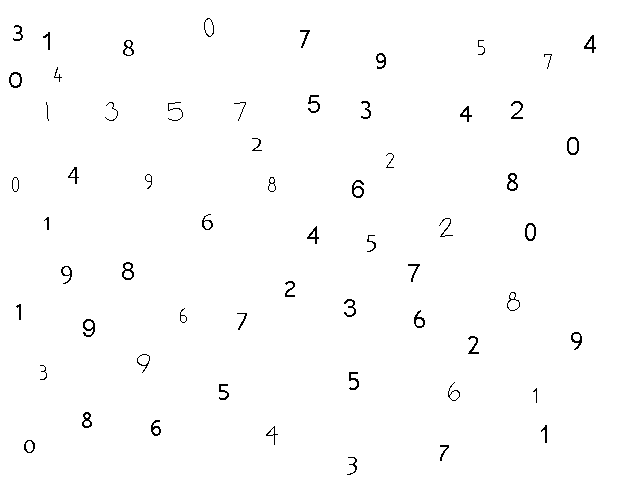
\includegraphics[scale=0.35]{test1}
\end{center}

Po przeprowadzeniu testu otrzymaliśmy zadowalający obraz wynikowy, który potwierdza, że stworzona przez nas 
sieć neuronowa działa i nadaje się do wykrywania prostych obiektów np liczb.

Oto otrzymany obraz wynikowy:

\begin{center}
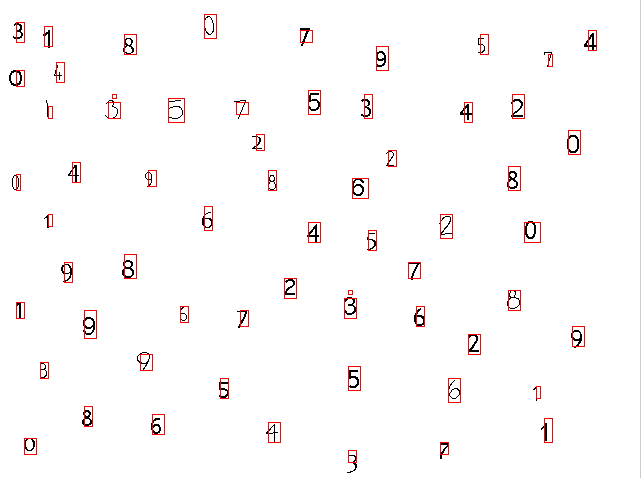
\includegraphics[scale=0.35]{wynik}
\end{center}

%=================================================
\newpage
\section{Rezultaty i wnioski}
Wykonując powyższy projekt natrafiliśmy na wiele problemów zarówno natury informatycznej, jak i matematycznej.
Większość z nich udało nam się rozwiązać samodzielnie, do pozostałych zaś rozwiązania znaleźliśmy w odpowiedniej
literaturze. Największego natomiast nie udało nam się w pełni rozwiązać. Nie mogliśmy dojść do tego, dlaczego
powstały przez nas algorytm nie chciał wykrywać twarzy, zaś cyfry wykrywał doskonale. Mieliśmy tutaj wiele teorii, 
które staraliśmy się po kolei eliminować. W końcu zaś skończyły nam się pomysły, bądź też brakło nam odpowiednich 
podstaw teoretycznych. Po konsultacji z opiekunem projektu postanowiliśmy skupić się w pełni na wykrywaniu cyfr na obrazie.
Z zadowoleniem możemy stwierdzić, że powstały przez nas algorytm  spełnia wyżej wspomniane zadanie.
Wykrywa on cyfry niezależnie od wielkości i ich ilości. 

Podczas realizacji projektu nauczyliśmy się wielu nowych i ciekawych rzeczy. Podejmując się wykonania projektu nikt
z nas nie miał pojęcia o tym czym są Sieci Neuronowe. Teraz zaś nie tylko znamy ich podstawy teoretyczne, ale także
potrafimy sami je zbudować i zaprojektować. Ponadto realizując projekt pogłębiliśmy naszą wiedzę z wielu innych dziedzin
informatycznych. Począwszy od nauki zaawansowanego programowania w Matlabie,
poprzez dokładniejsze poznanie metod przetwarzania obrazów cyfrowych, aż do poszerzenia umiejętności posługiwania się
informatycznymi narzędziami służącymi do pracy grupowej. 

Mamy nadzieję że to czego nauczyliśmy się podczas realizacji tego projektu zaowocuje w przyszłości 
i pozwoli nam się jeszcze bardziej rozwijać. Chociażby poprzez kontynuowanie projektu jako pracy inżynierskiej.

%=================================================
\section{Literatura}
 \begin{enumerate}
\item Convolutional Face Finder: A Neural Architecture for Fast and Robust Face Detection, 
Christophe Garcia and Manolis Delakis
\item Convolutional neural networks for image processing, Matthw Browne, Saeed Shiry Ghidary
\item An Embedded Robust Facial Feature Detector, Sebastien Roux, Christophe Garcia
\item Sieci Neuronowe, Ryszard Tadeusiewicz
 \end{enumerate}
%=================================================
\newpage
\section{Dodatek A: Opis narzędzi i metod postępowania}
\subsection{Implementacja algorytmu}
Działanie algorytmu wdrażaliśmy w środowisku MathWorks Matlab R2009b. Zdecydowaliśmy się na nie ze 
względu na mnogość łatwo dostępnych funkcji wspomagających obliczenia, szybkość implementacji oraz 
to iż w ciągu studiów nabyliśmy sporo doświadczenia przy pracy w nim, szczególnie przy obróbce 
grafiki.

Matlab posiada wbudowane narzędzia wspomagające pracę nad sieciami neuronowymi, ale niestety nie ma 
wśród nich obsługi konwolucyjnych sieci neuronowych. Dlatego też rozpoczęliśmy poszukiwania 
potrzebnych narzędzi w Internecie. Znaleźliśmy projekt Mikhail Sirotenki \footnote{ projekt dostępny
pod adresem  https://sites.google.com/site/mihailsirotenko/projects/convolutional-neural-network-class
[dostęp 10.06.2011]}  w którym wykorzystane zostały konwolucyjne sieci neuronowe do rozpoznawania 
odręcznie napisanych cyfr. Klasa odpowiedzialna za sieci neuronowe została napisana przez 
Yann LeCun'a. Początkowo modyfikowaliśmy skrypt dla naszych potrzeb, jednak po jakimś czasie 
uznaliśmy, że lepiej będzie go przepisać na nowo opierając się na pierwotnym z zachowaniem struktury
klasy. Zrzut ekranu okna programu Matlab:

\vspace*{0.5cm}
\begin{center}
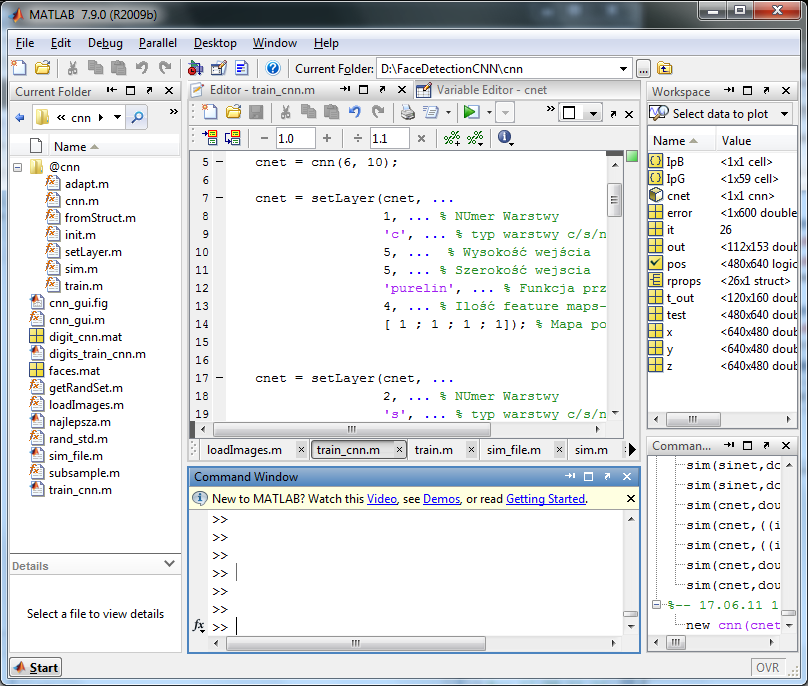
\includegraphics[scale=0.5]{matlab}
\end{center}
\vspace*{0.5cm}

Z prawej strony widać strukturę plików projektu. Folder @cnn zawiera pliki klasy cnn, zawierają 
między innymi konstruktor, funkcję treningową (\verb#train.m#), funkcję adaptacyjną 
(\verb#adapt.m#) oraz skrypt sprawdzający działania sieci neuronowej na podanym obiekcie 
(\verb#sim.m#).

Podstawowymi zadaniami jakie wykonaliśmy było wprowadzenie odpowiednich parametrów konwolucyjnych 
sieci neuronowych, przeprowadzenie treningu dla wybranych obrazów treningowych oraz analiza wyników 
działania sieci dla obrazów testowych po czym ponowna konfiguracja parametrów.

Aby rozpocząć naukę nowych sieci neuronowych należy uruchomić plik train\_cnn.m i poczekać na 
zakończenie treningu (wyświetli się wtedy wykres błędów). Aby przeprowadzić symulację 
wykorzystujemy skrypt sim\_file.m .

Podjęliśmy próbę użycia opracowanej przez firmę Nvidia architektury CUDA służącej do wspomagania 
obliczeń przy wykorzystaniu wydajnych układów graficznych. Niestety po zainstalowaniu pakietu 
deweloperskiego oraz potrzebnych bibliotek wciąz otrzymywaliśmy błędy o brakujących plikach, 
których z braku wiedzy o architekturze oraz dostępu do źródeł kodu nie udało nam się naprawić.
  

\subsection{Pozyskiwanie obrazów do treningu i testów}
Zdjęcia treningowe pochodzą z bezpłatnych baz zdjęć twarzy znalezionych w Internecie. Zdobyte 
zdjęcia zostały poddane ręcznej obróbce w edytorach grafiki GIMP, FastStone Image Viewer 4.5, 
MS Paint. Twarz należało odpowiednio przeskalować oraz wykadrować tak, aby nos znalazł się na środku
obrazka a cała twarz zmieściła się na obrazku o rozdzielczości 36x32.  Szczególnie przydatny był 
program IrfanView, którego użyliśmy do automatycznego, seryjnego przeskalowywania, zmiany nazw 
plików, konwersji do odcieni szarości i innych.

Obrazy nie przedstawiające twarzy (potrzebne w procesie nauki jako antywzorce) uzyskaliśmy poprzez 
pokrojenie obrazów krajobrazów oraz fragmentów zdjęć niezawierających twarzy. W tym celu napisaliśmy
w Matlabie skrypt slice.m, którego zadaniem jest utworzenie z jednego dużego wielu małych obrazków 
o zadanym rozmiarze.

\subsection{Organizacja pracy grupowej}

W celu realizacji projektu wielokrotnie spotykaliśmy się by wspólnie pracować. Po wyznaczeniu 
zakresu prac zaistniała potrzeba aby każdy z nas mógł pracować indywidualnie nad swoją częścią. Aby 
umożliwić równoczesną pracę zdalną skorzystaliśmy z rozproszonego systemu kontroli wersji GIT. 
Założyliśmy konta w ogólnodostępnym, w dużej części bezpłatnym serwisie github (https://github.com/)
oraz zainstalowaliśmy potrzebne oprogramowanie. Po utworzeniu repozytorium i przypisaniu członków 
można było bardzo szybko i łatwo nanosić swoje poprawki do projektu czy wysyłać pliki.

\vspace*{0.5cm}
\begin{center}
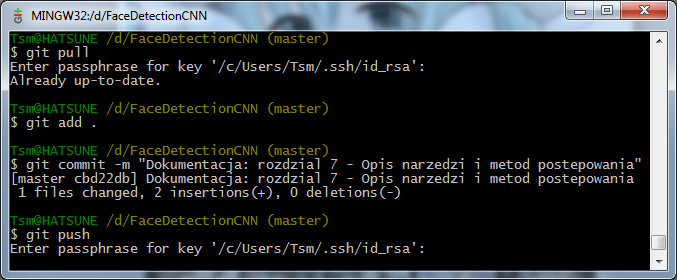
\includegraphics[scale=0.6]{gitconsole}
\end{center}
\vspace*{0.5cm}

W razie wystąpienia problemu można było przywrócić poprzednią, działającą wersję. Każdą, nawet 
drobną zmianę (tzw. commit) nalezało opisać komentarzem, co pozwalało wszystkich zorientować się 
co zostało zmienione.

\vspace*{0.5cm}
\begin{center}
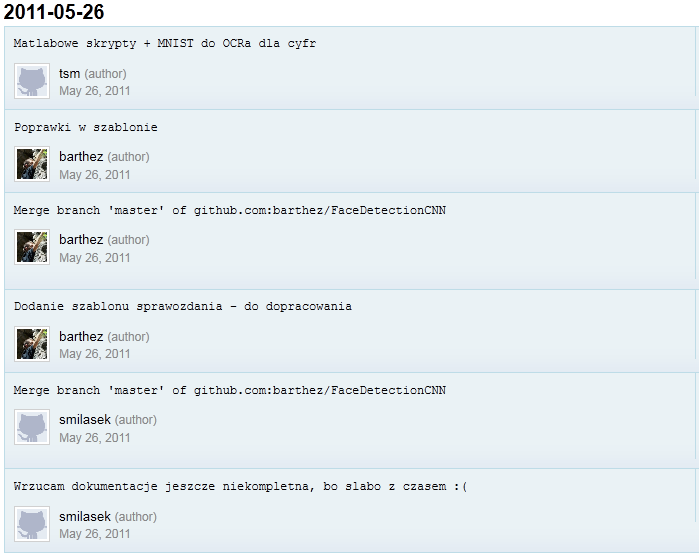
\includegraphics[scale=0.6]{commits}
\end{center}
\vspace*{0.5cm}

\subsection{Dokumentacja}

Niniejszą dokumentację stworzyliśmy w \LaTeX-ie przy użyciu programu MikTeX 2.9. Zdecydowaliśmy się na 
to, ponieważ \LaTeX umożliwia wstawianie skomplikowanych wzorów matematycznych, pozwala łatwo i 
szybko formatować tekst oraz wspomaga automatyczną indeksację treści i eksport do PDF. 


%=================================================
\section{Dodatek B: Opis obsługi programu}
 \begin{enumerate}
\item W programie Matlab należy otworzyć plik o nazwie \verb#train_cnn.m# znajdujący się w katalogu \verb#cnn#. Zamiast trenować sieci możemy wczytać zmienne z już wytrenowanymi sieciami, które znajdują się w plikach \verb#digit_cnn.mat#, \verb#face_cnn.mat# oraz \verb#face_cnn.2.mat#.
\item W pliku tym należy ustalić odpowiednie ścieżki dostępu do katalogów z obrazkami do nauki (zmienne  \textbf{IpG} i  \textbf{IpB})
\item Należy uruchomić zmodyfikowany skrypt Matlaba i poczekać do zakończenia procesu trenowania sieci 
(informacje o zakończeniu każdej z epok testowania pojawiają się w głównym oknie programu)
\item W workspace Matlaba powinna pojawić się nowa zmienna o nazwie cnet, która odpowiada wyuczonej przez nas sieci
\item Otwieramy plik o nazwie \verb#sim_file.m# i ponownie zmieniamy w nim ścieżkę do katalogu w którym znajdują się
obrazki do testów
\item Można także zmodyfikować zmienną  \textbf{debug} w zależności od tego czy chcemy obserwować kolejne
 etapy przechodzenia  obrazu testowego przez sieć neuronową
\item Odpalamy skrypt i obserwujemy wyniki.\\
Jeśli \textbf{debug} była ustawiona na 1, to obserwujemy w pierwszym oknie obrazy pośrednie. W przeciwnym wypadku
obserwujemy tylko realny wynik (wykrycie na obrazie pożądanych elementów)

 \end{enumerate}
%=================================================
\section{Dodatek E: Spis zawartości dołączonych nośników}

\end{document}
